\documentclass[12pt, a4paper]{article}
\usepackage{amsmath}
\usepackage{amsfonts}
\usepackage{amsthm}
\usepackage{mathtools}
\newtheorem{theorem}{Theorem}[section]
\newtheorem{definition}{Definition}[section]
\numberwithin{equation}{section}
\usepackage{pgfplots}
\pgfplotsset{width=10cm,compat=1.9}
\graphicspath{ {img/} }
\DeclareGraphicsExtensions{.png}

\title{word2vec}
\author{Kristian Wichmann}

\begin{document}
\maketitle

\section{A simple neural network}
Consider a feed forward neural network with one hidden layer, as shown in figure \ref{fig:nn}. The input layer consists of a row\footnote{Note that this is different from the column vector convention usually used.} vector $x$ of dimension $D_x$, i.e. $x\in\mathbb{R}^{1\times D_x}$. The hidden layer has $h$ neurons with a sigmoid activation function:
\begin{equation}
h=\sigma(xW^{(1)}+b^{(1)})=\sigma(z^{(1)}),\quad z^{(1)}=xW^{(1)}+b^{(1)}
\end{equation}
So $h\in\mathbb{R}^{1\times H}, W^{(1)}\in\mathbb{R}^{D_x\times H}, b^{(1)}\in\mathbb{R}^{1\times H}$. The output layer has $D_y$ softmax neurons:
\begin{equation}
\hat{y}=s(hW^{(2)}+b^{(2)})=s(z^{(2)}),\quad z^{(2)}=hW^{(2)}+b^{(2)}
\end{equation}
Similarly $\hat{y}\in\mathbb{R}^{1\times D_y}, W^{(2)}\in\mathbb{R}^{H\times D_y}, b^{(2)}\in\mathbb{R}^{1\times D_y}$.

\begin{figure}
\centering
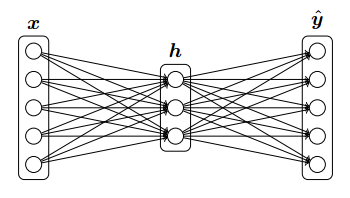
\includegraphics{w2v_nn}
\caption{The neural network.}
\label{fig:nn}
\end{figure}

\subsection{Error function}
Assuming a labelled dataset $x$ with the correct label $c$ encoded as a one-hot vector $t\in\mathbb{R}^{1\times D_y}$, so $t_i=\delta_{ic}$. We will use the cross-entropy error function:
\begin{equation}
J(x)=-\sum_{i=1}t_i\log\hat{y}_i
\end{equation}
Since $t$ is one-hot encoded, only the correct label $c$ will contribute to the sum, so:
\begin{equation}
J(x)=-\log\hat{y}_c
\end{equation}
This does not mean that the other components of $\hat{y}$ will not matter, since the softmax indirectly depends on all components.

\subsubsection{Derivative with respect to input}
We now wish to compute the derivative of $J(x)$ with respect to $x$. In shorthand, the chain rule gives us:
\begin{equation}
\frac{\partial J}{\partial x}=\frac{\partial J}{\partial\hat{y}}\frac{\partial \hat{y}}{\partial z^{(2)}}\frac{\partial z^{(2)}}{\partial h}\frac{\partial h}{\partial z^{(1)}}\frac{\partial z^{(1)}}{\partial x}
\end{equation}
Writing out indices explicitly:
\begin{equation}
\frac{\partial J}{\partial x_m}=\sum_{i=1}^{D_y}\sum_{j=1}^{D_y}\sum_{k=1}^H\sum_{l=1}^H\frac{\partial J}{\partial\hat{y}_i}\frac{\partial \hat{y}_i}{\partial z^{(2)}_j}\frac{\partial z^{(2)}_j}{\partial h_k}\frac{\partial h_k}{\partial z^{(1)}_l}\frac{\partial z^{(1)}_l}{\partial x_m}
\end{equation}
Let's compute these partial derivatives one by one:
\begin{equation}
\frac{\partial J}{\partial\hat{y}_i}=-\frac{\partial}{\partial\hat{y}_i}\log\hat{y}_c=-\frac{\delta_{ic}}{\hat{y}_c}
\end{equation}
The second is a standard result for the softmax function:
\begin{equation}
\frac{\partial \hat{y}_i}{\partial z^{(2)}_j}=s_i(z^{(2)})(\delta_{ij}-s_j(z^{(2)})=\hat{y}_i(\delta_{ij}-\hat{y}_j)
\end{equation}
And:
\begin{equation}
\frac{\partial z^{(2)}_j}{\partial h_k}=W^{(2)}_{kj}
\end{equation}
The fourth uses a standard result for the sigmoid:
\begin{equation}
\frac{\partial h_k}{\partial z^{(1)}_l}=\delta_{kl}\sigma(z^{(1)}_l)(1-\sigma(z^{(1)}_l))=\delta_{kl}h_l(1-h_l)
\end{equation}
And finally:
\begin{equation}
\frac{\partial z^{(1)}_l}{\partial x_m}=W^{(1)}_{ml}
\end{equation}
Inserting, letting the delta functions cancel, and renaming indices, this becomes:
\begin{equation}
\frac{\partial J}{\partial x_i}=-\sum_{j=1}^H\sum_{k=1}^{D_y}W^{(1)}_{ij}h_j(1-h_j)W^{(2)}_{jk}(\delta_{kc}-\hat{y}_k)
\end{equation}
But since $t_i=\delta_{ic}$ this is the same as:
\begin{equation}
\label{error_derivative}
\frac{\partial J}{\partial x_i}=\sum_{j=1}^H\sum_{k=1}^{D_y}W^{(1)}_{ij}h_j(1-h_j)W^{(2)}_{jk}(\hat{y}_k-t_k)
\end{equation}
We may rephrase this is terms of \textit{errors} for the different layers. The error in the output layer is:
\begin{equation}
\delta^{(2)}_k=\hat{y}_k-t_k
\end{equation}
And the backpropagated error in the hidden layer is:
\begin{equation}
\delta^{(1)}_j=\sum_{k=1}^{D_y}h_j(1-h_j)W^{(2)}_{jk}\delta^{(2)}_k
\end{equation}
Now equation \ref{error_derivative} can be rewritten as:
\begin{equation}
\frac{\partial J}{\partial x_i}=\sum_{j=1}^H\sum_{k=1}^{D_y}W^{(1)}_{ij}h_j(1-h_j)W^{(2)}_{jk}\delta^{(2)}_k=\sum_{j=1}^H W^{(1)}\delta^{(1)}_j
\end{equation}

\section{The word2vec algorithm}

\end{document}